\section{Pseudo-random generator - PRG}
\label{appendix:prg}

% AES counter mode

\begin{figure}[H]
    \centering

    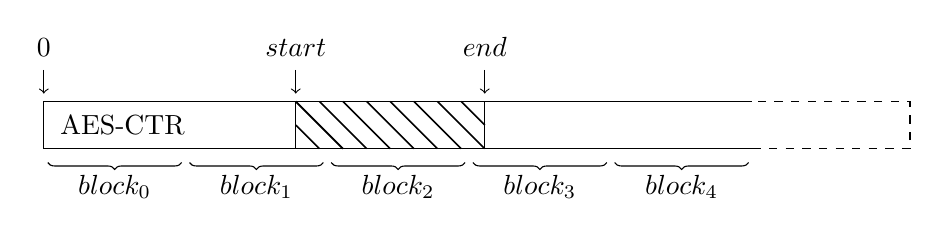
\begin{tikzpicture}
        \def\one{0.6}
        \def\width{9}
        \def\arrowstart{3.2}
        \def\arrowend{5.6}
        \def\padding{0.1}
        \def\arrowHeight{1}
        \def\dashLength{2}

        \draw (\width,0) -- (0,0) -- (0, \one) -- (\width,\one);
        \draw [dashed] (\width,0) -- (\width+\dashLength,0) -- (\width+\dashLength,\one) -- (\width,\one);

        \draw (1,\one/2) node {AES-CTR};

        \draw[->] (0,\arrowHeight) -- (0,\one+\padding)  node[above=10pt] {$0$};
        \draw[->] (\arrowstart,\arrowHeight) -- (\arrowstart,\one+\padding)  node[above=10pt] {$start$};
        \draw[->] (\arrowend,\arrowHeight) -- (\arrowend,\one+\padding) node[above=10pt] {$end$};

        \draw (\arrowstart,0) -- (\arrowstart,\one);
        \draw (\arrowend,0) -- (\arrowend,\one);


        \begin{scope}[shift={(\arrowstart,0)}]
            \def\a{2.4}
            \def\diff{1.8}
            \def\b{\one}
            \def\lw{0.2}

            \foreach \x [count=\i] in{0,0.3,0.6,...,\b}{
                    \draw [line width=\lw mm](\x,0)--(0,\x) (\a-\b+\x,\b)--(\a,\x);
                }
            \foreach \x [count=\i] in{0,0.3,0.6,...,\diff}{
                    \draw [line width=\lw mm](\x+\b,0)--(\x,\b);
                }
        \end{scope}

        \def\blockWidth{1.8}
        \foreach \i in{0,1,...,4} {
                \draw[decoration={brace,raise=5pt,mirror},decorate] (\i*\blockWidth+0.05,0) -- (\i*\blockWidth+\blockWidth-0.05,0) node[midway,below=6pt] {$block_{\i}$};
            }

    \end{tikzpicture}
    \caption{Pseudorandomness generator}
\end{figure}
